

\chapter{基于区域合并的图像显著性分析算法}
\label{cha:SGRM}
本章提出了一种显著性引导的图像区域合并算法,目标是直接通过区域合并的方式逐渐将图像从初始状态下的多个区域合并为显著性对象和背景2个区域。为实现这一目标,在不同的阶段采用不同的合并策略。首先利用超像素分割方法将图像分为若干初始区域。在第一阶段,仅合并相似且相邻的区域,使得属于同一对象的像素合并到同一区域。随后,处理上述过程中产生的空洞以及因遮挡造成的属于同一对象的区域不相邻的情况;随后,在区域显著分析的引导下,不断将显著性最差的区域合并到背景区域,而不是尝试将显著性区域合并到一起; 最后,利用合并过程中得到的多个候选显著性区域加权得到最终的显著性区域结果。 在2个公开测试集上进行了测试并与其它算法进行了对比,实验结果证明了本章所提算法的有效性,特别是在难度更大的ECSSD数据集~\cite{ECSSD}中,本章算法的准确度要优于其它同类算法。
\section{研究背景}
\label{sec:background}
图像显著性区域检测是近年来计算机视觉和图像处理领域的研究热点之一~\cite{saliencySurvey}。该技术的目标是快速定位图像中显著性对象,已经用于目标识别,基于内容的图像编辑以及图像检索等应用。早期的显著性检测算法~\cite{itti}依据视觉感知理论,采用自底向上方法预测人眼观察图像时的焦点(Fixation),得到一系列离散的圆点形状的显著性区域预测结果。然而,这类方法效率和准确度均较低,无法得到显著性对象的准确边界。随后,为了实现提前显著性对象的准确边界,研究人员提出了一系列数据驱动,自底向上的显著性区域检测算法~\cite{Achanta08,ChengPAMI,ufo,Yan2014Hierarchical},可以较为准确的提取自然图像中包含的显著性对象。\par
据文献~\inlinecite{Borji2015Salient}报道,在这些算法中,基于图像区域的算法性能更出色。基于区域的显著性检测算法首先用超像素~\cite{SLIC}、基于图的图像分割算法~\cite{graphseg}等图像分割方法将图像分为若干个小区域,随后以区域为单位进行显著性计算. 相比于基于像素的算法, 区域分割处理可以保持对象边界,同时利用区域颜色直方图可以更准确的对区域内的颜色对比度进行量化.另外,以区域为单位计算大大降低了运算量.这些算法的出发点都是根据显著性区域的特点,例如对比度高~\cite{ChengPAMI},处在相机焦点上~\cite{ufo}等,定义区域显著性模型,最终得到显著性区域结果。然而,自然图像中可能包含各种类型的显著性对象,单纯用这些线索仍然无法处理所有情况。如图~\ref{fig:saliencyCom}所示,(a)为输入图像,(b),(c),(d)分别为文献~\inlinecite{ChengPAMI},文献~\inlinecite{Yan2014Hierarchical}(CSH)算法和本章算法的结果,(e)为正确结果.图~\ref{fig:saliencyCom}表明,当输入图像中对象和背景的色彩分布较为接近(图~\ref{fig:saliencyCom}中第一行和第二行),或者背景复杂度较高(第三行)时RC和CSH算法均无法有效检测出显著性对象。
\begin{figure}[h]
  \centering%
      {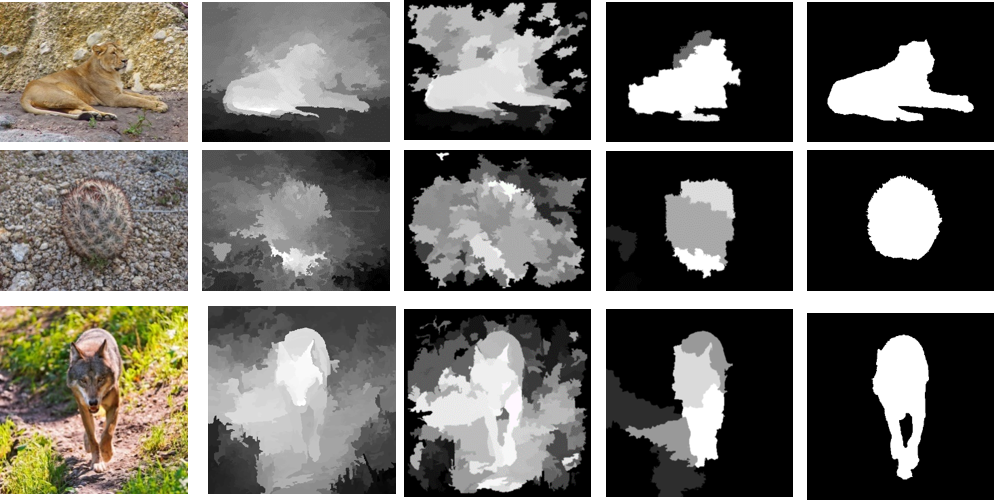
\includegraphics[width=0.9\textwidth]{ch02fig1.png}}\\
(a)\quad\quad\quad\quad\quad
(b)\quad\quad\quad\quad\quad\quad
(c)\quad\quad\quad\quad\quad\quad
(d)\quad\quad\quad\quad\quad
(e)
  \caption{显著性检测结果对比}
  \label{fig:saliencyCom}
\end{figure}

\par
为了解决这一问题,本章将显著性区域检测问题视为图像分割问题,以显著性引导的区域合并的方式将图像分为显著性区域(前景)和背景两个区域。在合并过程中采用了与主流基于区域的图像显著性检测算法~\cite{Achanta08,ChengPAMI,ufo,Yan2014Hierarchical}相反的策略,即不再尝试定位显著性区域,而是利用背景线索来估计背景区域,并不断将显著性差的非前景区域合并到背景区域。根据观察,大部分自然图像中的背景部分的像素具有连续性强的特点~\cite{huamiao},例如室外拍摄图像中的天空,地面等背景区域。此外,图像的边缘部分应该大部分都是背景~\cite{backgroundPrior}。如果不断将图像中相似的小区域进行合并,背景部分像素应该更容易合并到一起,并且将包含更多的图像边缘.观察图~\ref{fig:saliencyCom}中输入图像的背景部分,如第一行图像中的地面以及狮子身后的山、第二行图像中的石块地面、以及第三行图像中的草地,虽然这些背景部分色彩分布与前景接近或者具有较高的复杂度,其仍然具有这种较强的连续性。利用这一特点,我们首先将图像进行超像素分割,随后在区域显著分析的引导下不断将显著性最差的区域合并到背景区域,而不是尝试将显著性区域合并到一起。 最后,利用合并过程中得到的多个候选显著性区域加权得到最终的显著性区域结果。将本章算法在两个公开的数据库ASD[9]和ECSSD[5]中的共计2000张图像中进行了测试并与其它算法进行了对比,实验结果验证了本章所提算法的有效性.在较为困难的ECSSD测试集中,本章算法得到的F-Mearsure以及平均绝对误差(Mean Absolute Er-ror,MAE)均优于其它参与比较的算法.

\section{相关工作}
\label{sec:relatedWorks}
\subsection{图像显著性区域检测}
\label{sec:SaliencyDetection}
对比度(contrast)强是显著性对象区别于背景的重要性质,Cheng等人~\cite{ChengPAMI}提出利用全局对比度的方法计算图像中每个颜色的显著性水平。由于色彩空间巨大,为了提高效率,Cheng等人提出量化的方式提取图像中的主要颜色并依据此建立直方图,计算每个颜色的显著性值。为了进一步提高算法的准确的,Cheng等人~\cite{ChengPAMI}提出了一种基于区域对比度的方法,先用基于图的图像分割方法将图像分为若干齐次区域,考虑区域的空间相关性,利用区域对比度来检测显著性区域,得到了比全局对比度更好的效果。Perazzi等人~\cite{saliencyFilter}提出基于高维高斯滤波的显著性滤波算法(saliency filters)。该算法首先对待处理图像进行抽象化,去掉冗余细节信息;在CIELab色彩空间中通过局部及全局对比度来计算色彩独特性,利用高维高斯滤波的方式结合色彩的空间分布情况计算最终的显著性检测结果。Jiang等人~\cite{ufo}指出,作为主要目标显著性对象应该在成像时处于相机焦点之上,利用图像中边缘的模糊程度可以对图像区域是否在成像时处于相机的焦点上进行量化,最后综合考虑图像区域对比度、是否在相机焦点上以及区域中包含对象的可能(objectness)三方面线索计算最终的结果。为了处理自然图像中的复杂结构,Yan等人~\cite{ECSSD}提出了一种多尺度参差花的显著性区域检测算法(CSH),该方法将图像在不同尺度上进行分割,得到多个层次的区域显著性线索,并将这些多层次的线索进行加权得到最终结果。本章所提出的方法与CSH算法有类似之处,均采用了图像区域合并的方法得到多个图像分割结果。但不同之处在于本章提出的区域合并方法在合并过程中的不同阶段使用不同的合并策略,而CSH算法使用同样的分层策略得到固定数量的层次。并且,本章使用背景线索进行区域显著性分析,与上述基于显著性对象线索的算法均不同。\par
Wei等人~\cite{geodesicDistance}提出了一种基于背景线索的显著性检测算法,该方法利用背景部分像素容易连接到图像边界的特点,利用图像区域距离图像边界的测地线距离(geodesic distance)来评估其显著性.文献~\inlinecite{backgroundPrior}中利用了图像边界大部分是背景这一假设,先对图像边界区域进行对比度分析,从中获得背景区域主要颜色的线索;随后利用这一线索利用基于~\ inlinecite{ChengPAMI}的算法进行对比度分析获得显著性前景结果。本章算法基于类似的背景线索,但是本章所提算法通过显著性引导的区域合并的方式进行显著性检测,这与文献~\inlinecite{geodesicDistance,backgroundPrior}有较大差别。

\subsection{图像区域合并}
\label{sec:regionMerging}
图像区域合并是指根据图像区域之间的相似性,逐渐将相似的区域合并在一起的过程,常用于图像分割等应用中。Richard~\cite{Richard2004Statistical}提出了一种基于统计的区域合并的提醒分割算法,利用图像统计特许确定需要合并的区域以及合并的顺序。文献~\inlinecite{Xiao2015Complexity}提出了一种复杂度自适应的图像区域距离以衡量图像区域的相似性,并基于此进行区域合并。最后根据区域中包含边缘信息的来评估区域中包含对象的可能性。文献~\inlinecite{SelectiveSearch}中提出了一种基于贪心算法的图像区域合并方法,该方法不断合并所有邻居区域中最接近的两个区域,直到将整幅图像合并为一个区域。上述区域合并方法作为预处理方法用于对象识别和显著性区域检测算法中取得了不错的效果。但上述方法均在区域合并过程中均始终采用同一策略,没有考虑到区域合并过程中不同阶段的不同特点,容易将属于对象的像素合并到背景区域。与这些方法不同,本章所提算法的目标是将图像分为显著性对象和背景2个区域,且在不同的阶段采用不同的合并策略,可以避免在合并过程中误将显著性对象合并到背景区域。

\section{算法描述}
\label{sec:algorithm}
本章算法主要分为三个阶段,主要流程图见图~\ref{fig:algflow}所示。首先,依据像素的空间相关性和色彩一致性利用文献~\inlinecite{superpixel}的算法对图像进行超像素分割, 将图像分为多个初始区域。 随后开始第一阶段合并,在此阶段不断将相似的相邻区域进行合并,直到区域数量达到阈值$N$。由于前景的遮挡,可能会使某些背景区域被分割成多个小区域,同时在前一过程中会有一些小区域由于与周围区域差别较大无法参与合并而形成空洞。在第二阶段处理这些遮挡和空洞问题,允许相似但不相邻的区域进行合并,同时将空洞区域与其最相似的邻居区域进行合并。在第三阶段,采用显著性引导的合并策略,分析各区域的显著性,将显著性最差的区域标记为背景区域$R_{B}$,剩下的其它区域一起可以看作是可能的显著性区域。不断以显著性从低到高的顺序依次将所有区域合并到$R_{B}$。最后将在合并过程中可以得到的候选显著性区域(Proposals)加权平均得到最终显著性区域结果。\par
\begin{figure}[h]
  \centering%
      {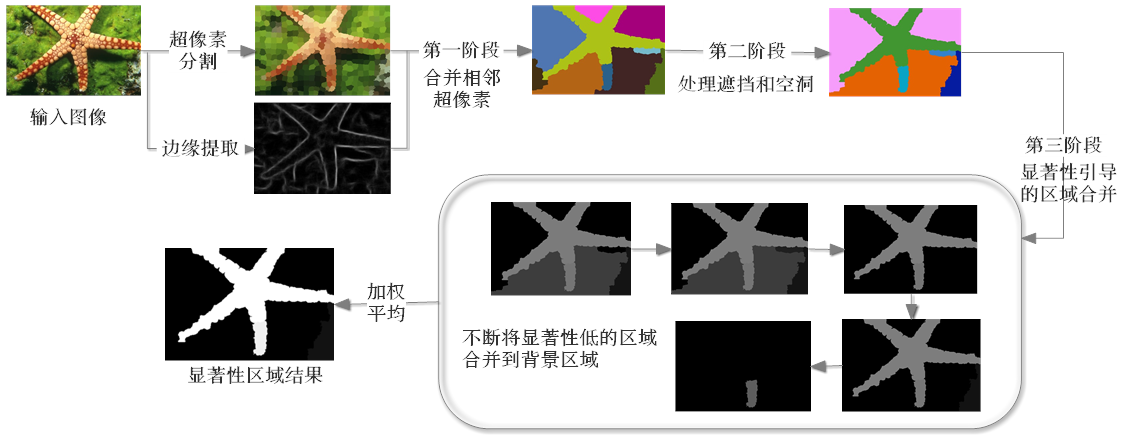
\includegraphics[width=0.9\textwidth]{SGRMflowChart.png}}

  \caption{算法流程图}
  \label{fig:algflow}
\end{figure}

\par
下面分别详细介绍各阶段的合并规则。

\subsection{第一阶段合并}
\label{subsec:mergeP1}
第一阶段合并只允许相似且相邻的区域进行合并。将区域$i$与区域$j$的合并优先级定义为$PR(i,j)$。计算区域合并的优先级时考虑以下四项因素。
\begin{itemize}
\item (a)颜色相似性\par
    直观上看,色彩分布一致的区域属于同一对象的概率很大。利用区域颜色直方图的巴氏距离(bhattacharyya distance)来量化区域之间的色彩相似性,越相似的区域合并优先级越高。

    \begin{equation}
    \label{equ:chap2:Pc}
    P_{c}(i,j)=1-HistogramDist(i,j)
    \end{equation}
    其中HistogramDist为计算直方图巴氏距离的函数。为了提高效率,利用文献~\inlinecite{ChengPAMI}的算法建立量化直方图,在保证覆盖$95\%$以上像素颜色的情况下,去掉图像中出现频次较低的颜色,从而减少直方图的分块(bin)数量,以减少计算量。
\item (b)边缘保持\par
    图像结构化边缘是反映对象边界的重要信息。为了使区域合并过程不破坏对象的边界,在合并优先级中加入边缘保持项,降低区域间的边界包含图像边缘的区域对的优先级。具体其定义为:
    $$P_{e}(i,j)=1-\frac{E(i,j}{min(borderLen(i),borderLen(j)}$$
    其中$E(i,j)=\sum_{b\in border(i,j)}Edgeness(b)$,即区域$i$和$j$之间的边界的边缘响应之和, $borderLen(i)$表示区域$i$的边界的长度(像素数)。我们利用文献~\inlinecite{DollarEdge} 的算法计算图像的结构化边缘响应,并将其归一化到$[0,1]$之间。
\item (c) 区域空间相关性\par
    区域的空间相关性指区域在空间上的关联性,对于相邻的区域其相关性定义为$P_{s} (i,j)=borderLen(i,j)/min⁡(border(i),border(j)$,其中 $borderLen(i,j)$表示区域$i$和$j$之间边界的长度。区域空间相关性的几何意义为若两区域之间的边界占比越大,说明两区域在空间关系上关联更紧密,因此合并优先级更高。极限情况下,当区域$i$ 完全包含$j$时$P_{s} (i,j)=1$。
\item (d) 区域面积\par
    为了使区域合并在图像全局范围内进行,对面积较小的区域赋予较大优先级,其定义为:
    $$P_{si}=1-(size(i)+size(j))/TotalSize$$.

\end{itemize}
最终, $PR(i,j)$由上述四项加权平均得到:
\begin{equation}
   \label{equ:chap2:PR}
   PR(i,j)=w_{c}\times P_{c}+w_{e} \times P_{e} + w_{s} \times P_{s} + w_{si} \times P_{si}
\end{equation}
其中加权系数$w_c=0.5, w_e=0.1, w_s=0.2, w_si=0.2$为固定值。\par

第一阶段合并过程的具体算法如下:



\renewcommand{\algorithmcfname}{算法}
\begin{algorithm}
\LinesNumbered
\KwData {初始化区域$Regions$,每次合并的区域比例$k$ ,区域合并目标数$N$ }
\KwResult {合并后的区域$Regions$}
 \While {Size(Regions) > $N$}{
    对每一组相邻区域$i,j$,用公式\ref{equ:chap2:PR}计算合并优先级$PR(i,j)$\;
    根据优先级从大到小对相邻区域对进行排序\;
    选取前面$k\times Size(Regions)$个相邻区域对进行合并\;
    更新区域信息和区域大小\;}

\label{algMergeP1}
\caption{第一阶段合并算法}
\end{algorithm}

\subsection{遮挡和空洞处理}
\label{subsec:mergeP2}

由于前景的遮挡,背景区域通常被分割为多块不相邻的区域,例如图\ref{fig:algflow}中的背景部分,而这些背景部分应该用一个区域表示更合理。在第一阶段的合并中并不允许不相邻的区域合并,防止在早期将那些属于前景但与局部背景接近的区域合并到背景中。在第一阶段合并结束之后处理遮挡则可以有效避免这一错误。遮挡处理的算法为:
\renewcommand{\algorithmcfname}{算法}
\begin{algorithm}
\LinesNumbered
\KwData {图像区域$Regions$, 合并门限$Threshold$ }
\KwResult {合并后的区域$Regions$}
    计算Regions中的各区域之间的平均颜色直方图距离avgDist\;
    //寻找颜色直方图距离最小的两个区域minI,minJ\;
    minDist = FindMinDist(Regions,minI,minJ)\;
    MaxDist = avgDist*Threshold\;
    \While{$minDist < MaxDist and Size(Regions)>2$}{
	   合并minI, minJ\;
        更新Regions\;
        minDist =FindMinDist(Regions,minI,minJ)\;}


\label{algMergeP2}
\caption{遮挡处理}
\end{algorithm}

\subsection{显著性引导的区域合并}
\label{subsec:mergeP3}

在前两个阶段完成后,图像中属于同一对象的像素已经合并到了同一个区域中。本章算法的目标是继续进行区域合并,将图像分为显著性区域和背景区域。与其它大部分基于显著性对象独特性算法不同,本章算法从背景线索入手,不断地将显著性低的区域合并到背景区域。根据观察和实验验证,属于背景的区域主要特点有:
\begin{itemize}
\item (a)连续性强,与周围区域相似度高~\cite{geodesicDistance};
\item (b)靠近图像的边缘~\cite{backgroundPrior};
\item (c)背景区域之间的对比度相对于前景对象较低~\cite{geodesicDistance}。
\end{itemize}

根据(a)和(b),可以推断背景区域易在第一阶段和第二阶段的合并中被合并到包含图像边缘的区域中。因此,选取包含图像边缘像素最多的区域作为背景区域$R_B$.定义区域的显著性值为:
\begin{equation}
   \label{equ:chap2:Saliency}
   Saliency(i)=k_b \times (1-BorderR(i))+ k_a \times (1-AD2c(i)) + k_c \times ContrastB(i)
\end{equation}
其中,$BorderR(i)$表示区域i中属于图像边缘的像素占全部图像边缘的比例,$ContrastB(i)=HistogranDist(H(i),H(R_B ))$,即区域$i$与背景区域$R_B$的颜色直方图距离。 $AD2c(i)$为区域$i$中心与图像中心的平均距离,归一化到$[0,1]$范围。在大多数情况下,摄影师在拍摄照片时都会将主体放在靠近中心的位置,因此靠近图像边缘的部分是背景的概率较大。加权系数$k_b k_a,k_c$为常量,它们的值分别为0.3,0.3,0.4。\par
第三阶段合并的算法如下所示:
\renewcommand{\algorithmcfname}{算法}
\begin{algorithm}
\LinesNumbered
\KwData {图像区域$Regions$, 背景区域$R_B$ }
\KwResult {候选显著性区域Proposals}

    \While{$Size(Regions)>2$}{
	   利用公式\ref{equ:chap2:Saliency}计算Regions中每个区域$i$的显著性值S(i)\;
        寻找显著性值最小的区域$minR$\;
        将minR合并到$R_B$\;
        $Proposal = \forall R \in Regions, R \neq  R_B$ \;
        将Proposal添加到Proposals\;}


\label{algMergeP2}
\caption{显著性引导的区域合并}
\end{algorithm}

\section{显著性区域检测}
\label{sec:saliency}

在自然图像中,前景通常可认为是由多个部分组成,例如人的身体通常可分为皮肤部分、衣服、裤子等。这些部分的颜色和纹理信息等有着较大差别,在合并时很难合并到一起。为了得到完整的显著性区域,将第三阶段合并过程中产生的非背景区域作为候选显著性区域。假设候选区域$Proposals(i)$包括$k_i$个区域,其中区域$j$的显著性值$PropSal(i,j)$定义为:
$$
   PropSal(i,j)=ContrastB(j) \times \exp{(-\frac{Ad2c(j)^2}{\varphi_d^2 })}
$$
其中,$\varphi_d=0.33$为固定值。\par
在合并过程中可以得到多个候选显著性区域,综合考虑候选区域的对比度、形状以及大小等因素对每个候选区域进行可靠性评估,其可靠性值定义为:
\begin{equation}
   \label{equ:chap2:PropSal}
   PropCon(i,j)=w_o \times Obj(i) + w_f \times Fillness(i) + w_sc \times Scale(i)
\end{equation}
其中, $Obj(i)$用于评估区域中包含对象的可能性(Objectness)\cite{objectness},具体定义为:
$$Obj(i) = HistogramDist(H(i),H(BoxBorder(i)))$$
设$BB(i)$为包围$Proposals(i)$的最小矩形.上式中$H(BoxBorder(i))=Histogram(p), p \in BB(i)-Proposals(i)$,表示位于$BB(i)$之内区域$Proposals(i)$之外的边界部分像素的直方图。公式\ref{equ:chap2:PropSal}中的$Fillness$定义为:
$$ Fillness(i) = \exp({-(\frac{size(i)}{size(BB(i))}-m_f)^2}/\varphi_f^2)$$ \par

在一般情况下,显著性区域一般形状较为紧凑,假如候选区域中还包括背景区域则会使得$Fillness$值较小。本章中$m_f,φ_f$分别为0.56和0.33。 公式\ref{equ:chap2:PropSal}中的最后一项为尺度可靠性,定义为$Scale(i)= \exp(-(size(i)- m_s)^2/\varphi_s^2)$,主要评估显著性区域大小的可靠性,在大多数情况下显著性区域一般只占整个图像的局部,假如候选区域过大则说明其中还包括未合并到背景中的非显著性区域;而如果候选区域过小则说明其可能仅是前景的一部分。本章中$m_s,φ_s$分别为0.3和0.5。\par

最后,依据$P$个候选显著性区域及其可靠性指标,以加权平均的方式得到最终显著性结果:
$$ S(I) = \frac{\sum_{i=1}^{P}Con(i) \times \sum_{j=1}^{k_i}PropSal(i,j)}{\sum_{i=1}^{P}Con(i)}$$


\section{实验结果与分析}
\label{sec:results}
通过C++编程借助OpenCV~\cite{opencv_library}实现了本文算法,在两个公开的测试集ASD~\cite{Achanta08}和ECSSD~\cite{ECSSD}上进行了测试。两个数据集中均包含1000张图像。其中ECSSD数据集中的图像主要是自然场景下拍摄的图像,其背景复杂度相比于ASD数据集中的图像更高,同时也更接近日常实际应用。这两个数据集中均包含人工标注的精确显著性区域。\par
在实验中, 算法~\ref{algMergeP1}中的参数设置为$k=0.2,N=15$,算法~\ref{algMergeP2}中的$threshold=0.8$。公式~\ref{equ:chap2:PropSal}中的系数$w_o,w_f,w_sc$分别为0.3、0.05、0.65,在本章所以实验中上述所有参数均使用固定值。将本章所提出的算法 (RM)与AC~\cite{Achanta08},CSH~\cite{Yan2014Hierarchical},FT~\cite{saliencyFilter},GB~\cite{Harel07graph-basedvisual},GC~\cite{GC},GMR~\cite{GMR},IT~\cite{itti},RC~\cite{ChengPAMI}, SF~\cite{saliencyFilter},SR~\cite{SR}方法进行了比较。其中RC、GMR、CSH算法和本文算法都属于基于区域的方法。部分结果的比较见图~\ref{fig:chap2:comp1}和图~\ref{fig:chap2:comp2}。通过对比可以看到,本文算法可以处理各种复杂背景的自然图像,例如图~\ref{fig:chap2:comp1}中的第三行以及图~\ref{fig:chap2:comp2}中的第二行,对于这些类型的图像RC等算法无法有效工作。而对于背景部分与前景部分在色彩空间分布较为接近的情况,例如图~\ref{fig:chap2:comp1}中的第二行及图~\ref{fig:chap2:comp2}中的第三行,本文算法的处理结果同样优于基于全局对比度的RC等算法。\par
\begin{figure}[h]
  \centering%
      {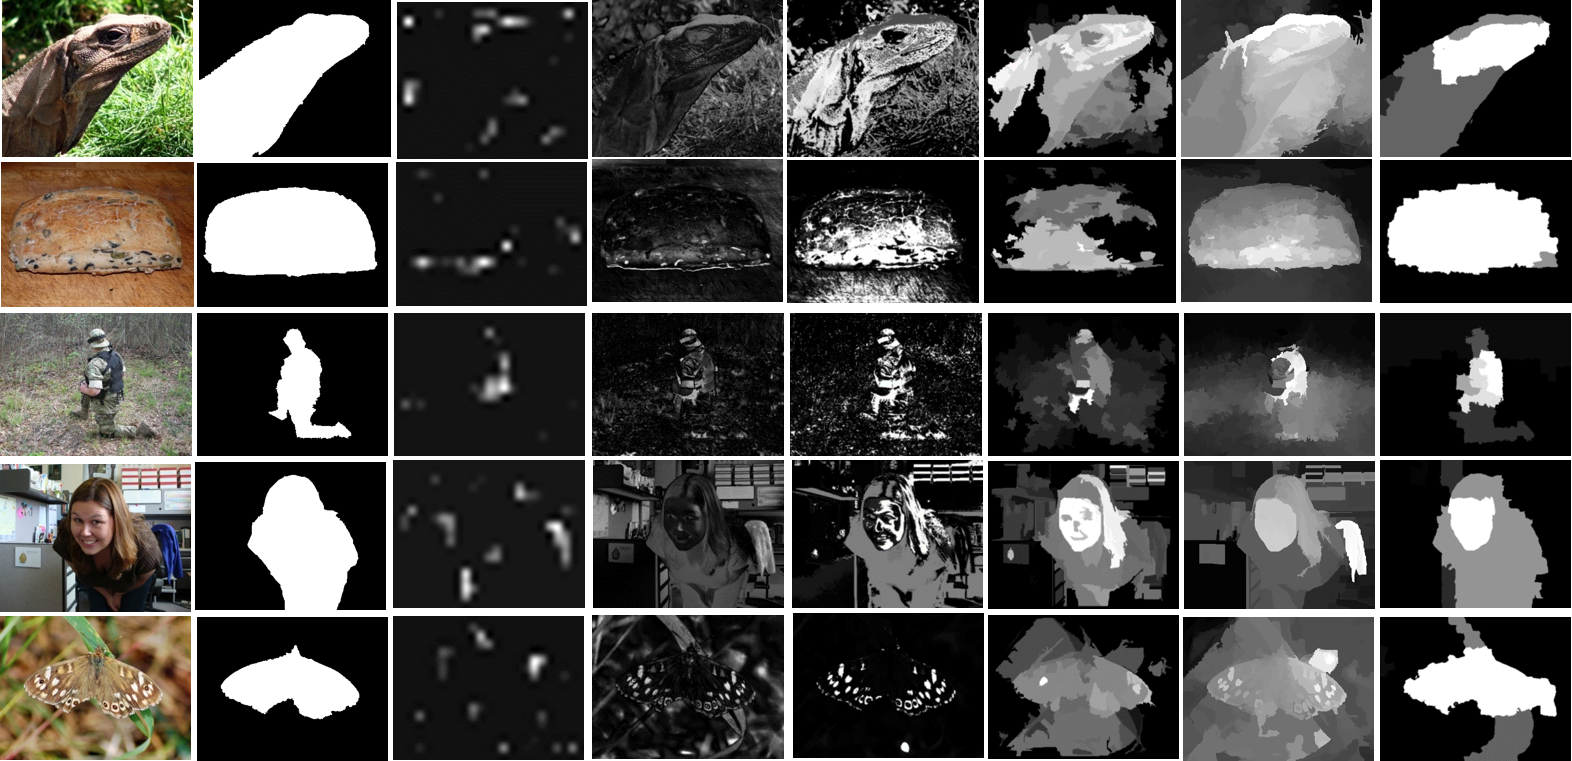
\includegraphics[width=0.9\textwidth]{salcomp1.png}}

  \caption{ECSSD数据集部分图像显著性检测结果比较}
  \label{fig:chap2:comp1}
\end{figure}
\begin{figure}[h]
  \centering%
      {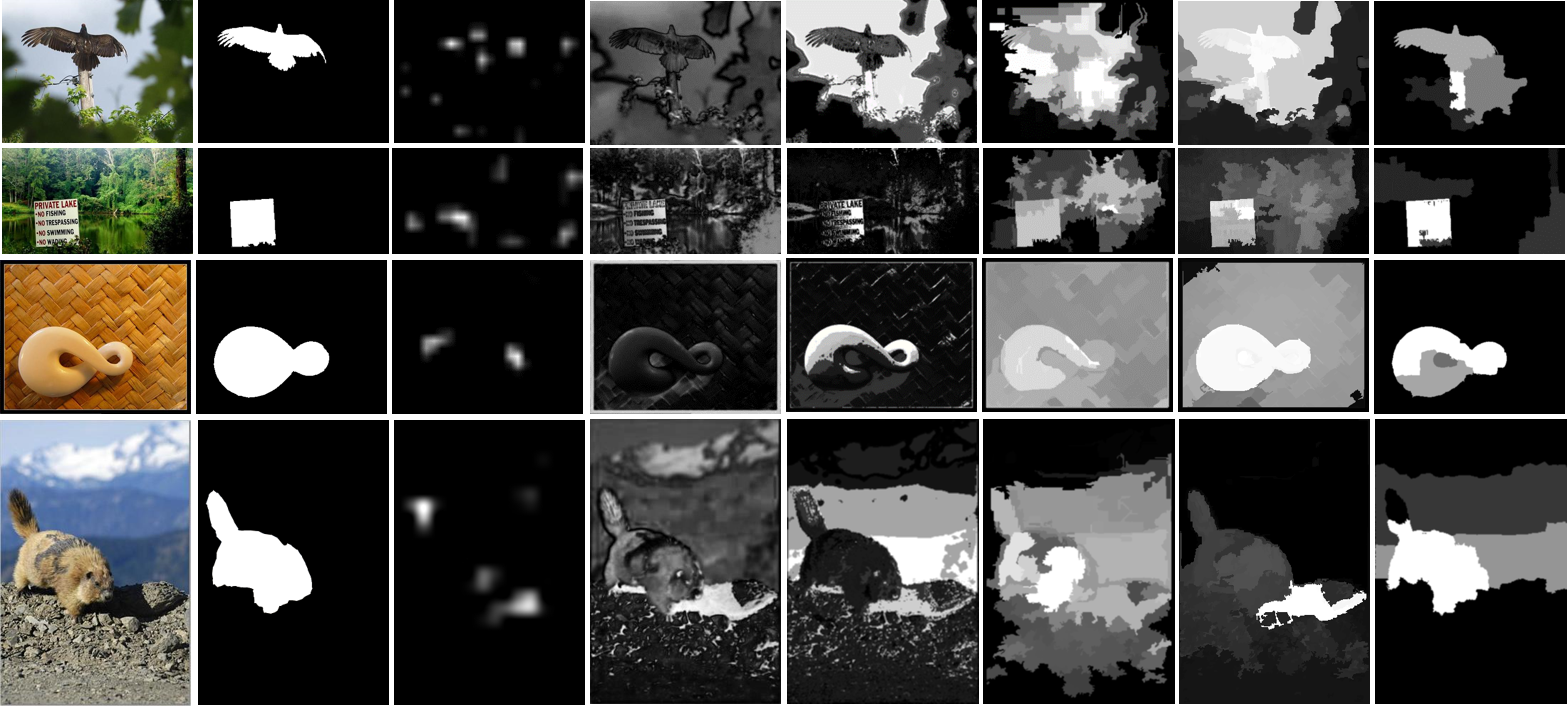
\includegraphics[width=0.9\textwidth]{salcomp2.png}}

  \caption{ASD数据集部分图像显著性检测结果比较}
  \label{fig:chap2:comp2}
\end{figure}
为了定量衡量算法的准确性,将显著性检测结果进行二值化后得到的显著性对象与数据集中提供的正确结果进行对比,本文采用通用的F-Measure值指标来比较算法准确性,其定义为:
$$F_{\beta} = \frac{(1+\beta^2)Precision \times Recall}{\beta^2 \times Precision + Recall}$$
其中$Precision$为精度,$Recall$表示召回率,$\beta^2=0.3$. \par

在实验中,为了消除二值化阈值对结果的影响,将阈值设定为在0到255之间变化,绘制F-Measure随阈值变化的曲线,见图~\ref{fig:sub:ecssdFCurve}和图~\ref{fig:sub:asdFCurve},同时图~\ref{fig:sub:ecssdAvg},~\ref{fig:sub:asdAVG}统计了各方法得到的F-Measure平均值和最大值。通过比较可以看出,本章算法在ECSSD数据库中的F-Measure平均值和最大值均优于其它算法,在ASD数据库中得到的平均F-Measure高于GMR算法外的其它算法。本文算法得到的F-Measure曲线较为扁平,即F-Measure取值受阈值影响较小。当阈值在128附近时F-Measure可以得到最大值。比较两个数据集,可以发现ASD数据集中的部分图像背景复杂度较低,因此各算法在ASD数据集上的测试结果均优于ECSSD数据集上的结果。由于本文算法的结果是通过区域合并得到的,只有超像素级精度,这使得本文算法在ASD数据库中得到的结果的精度要略低于GMR,RC等算法。 \par
$MAE$是另一个衡量显著性区域检测结果准确性的指标,其定义为:
$$MAE=1/(W\times H) \sum_{x=1}^W\sum_{y=1}^H \| S(x,y)-G(x,y)\|$$ ,其中$W,H$分别为图像的宽和高,$S$为显著性检测结果,$G$为正确值,两者均归一化在[0,1]之间。MAE值越低说明显著性检测误差越小,图~\ref{fig:sub:MAERst}是各算法MAE值在两个数据库中的比较结果。本文算法同样在ECSSD数据库中优于其它算法,在ASD数据库中略高于MAE最低的GMR算法。\par
\begin{figure}[h]
  \centering%
  \subcaptionbox{F-Measure曲线\label{fig:sub:ecssdCurve}} %标题的长度,超过则会换行,如下一个小图。
    {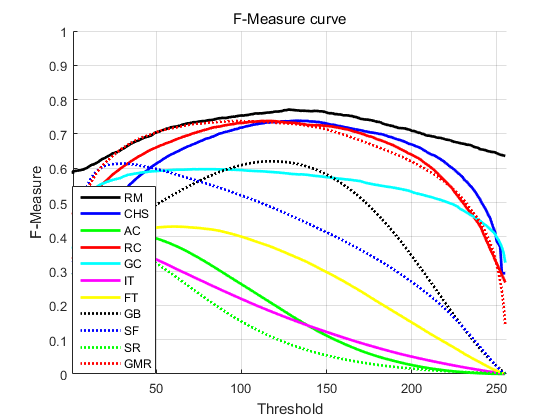
\includegraphics[width=0.45\textwidth]{ECSSD_FCurve}}%
 %\hspace{1em}%
  \subcaptionbox{平均F-Measure\label{fig:sub:ecssdAvg}}
      {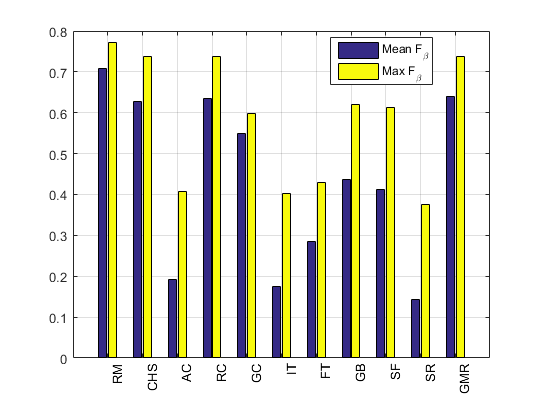
\includegraphics[width=0.45\textwidth]{ECSSD_FBar.png}}
  \caption{ECSSD数据库F-Measure值比较}
  \label{fig:ECSSDRst}
\end{figure}

\begin{figure}[h]
  \centering%
  \subcaptionbox{F-Measure曲线\label{fig:sub:asdCurve}} %标题的长度,超过则会换行,如下一个小图。
    {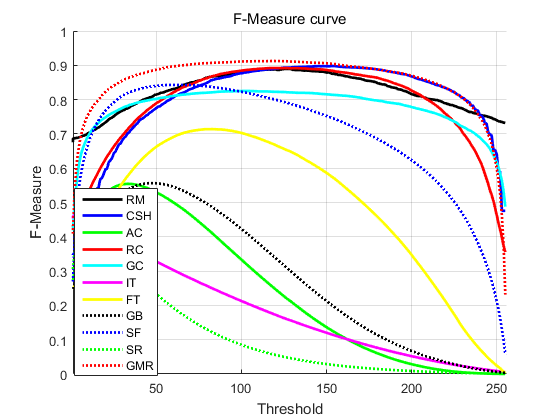
\includegraphics[width=0.45\textwidth]{ASD_FCurve}}%
 %\hspace{1em}%
  \subcaptionbox{平均F-Measure\label{fig:sub:asdAvg}}
      {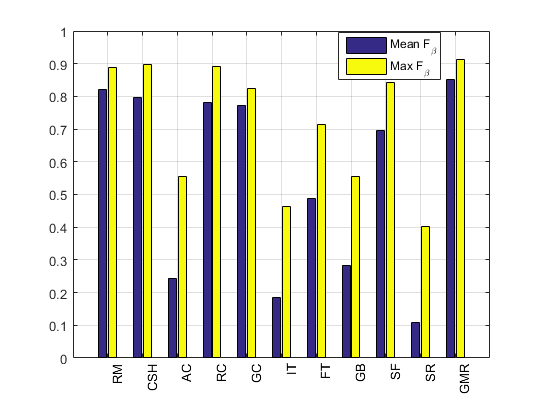
\includegraphics[width=0.45\textwidth]{ASD_FBar.png}}
  \caption{ASD数据库F-Measure值比较}
  \label{fig:ASDRst}
\end{figure}

\begin{figure}[h]
  \centering%
  \subcaptionbox{ECSSD数据集结果\label{fig:sub:ecssdMAE}} %标题的长度,超过则会换行,如下一个小图。
    {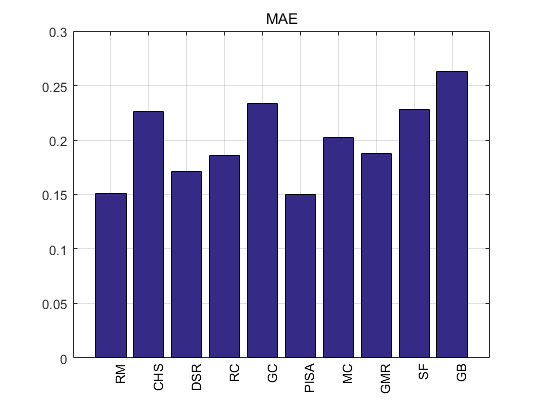
\includegraphics[width=0.45\textwidth]{ECSSD_MAE.png}}%
 %\hspace{1em}%
  \subcaptionbox{ASD数据集结果\label{fig:sub:asdMAE}}
      {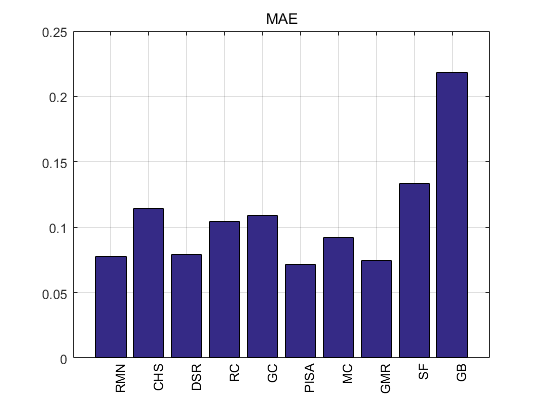
\includegraphics[width=0.45\textwidth]{ASD_MAE.png}}
  \caption{算法MAE比较}
  \label{fig:MAERst}
\end{figure}

部分算法的速度比较见表1.所列数据在配备Intel i7 3.5GHz CPU,16GB RAM的电脑上测得,参与比较的算法均用C++语言实现,其中CSH,RC和GMR算法均使用作者公开的代码进行测试。ASD数据库和ECSSD数据库中图像大小平均约为400×300,表中所列时间为处理每幅图像所用的平均时间。本文算法的速度相比RC和GMR算法稍快,比CSH算法快4倍左右。\par


虽然本文算法可以处理部分复杂背景的情况,但在处理背景连续性较差的图像时效果较差,主要原因是在区域合并的过程中会将前景区域错误的合并到背景中,从而无法提取到正确的前景.例如,在图8中,前两列为输入图像和正确前景,后三列分别为本文算法第一阶段,第二阶段合并结果以及最终提取的显著区域结果.由于这两幅图像中的背景部分十分复杂,并不具备本文假设的连续性,因此在区域合并时误将前景区域合并到了背景中,导致算法失败.
 \begin{figure}[h]
  \centering%
      {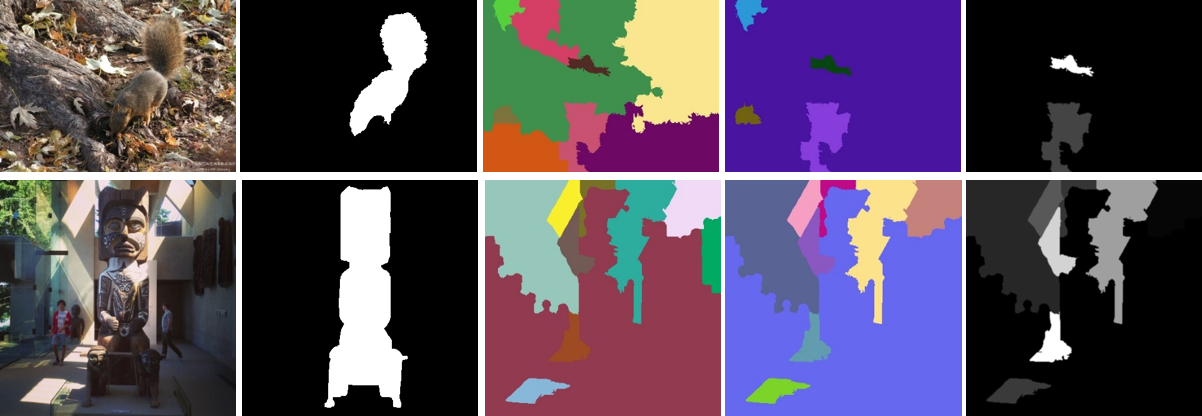
\includegraphics[width=0.9\textwidth]{fail.png}}

  \caption{本文算法部分失败例子}
  \label{fig:chap2:comp1}
\end{figure}


\section{本章小结}
本文以将图像分为显著性对象和背景2个区域为目标,提出了一种显著性引导的区域合并算法.由于在区域合并的不同阶段采取了不同的合并策略,本文算法能有效的防止在合并过程中将前景显著性对象错误的合并到背景区域.为了得到显著性对象,本文利用背景线索进行区域显著性分析,不断将非显著性区域合并到背景区域.将合并过程中得到的非背景区域作为候选显著性区域,通过加权平均的方式得到最终结果.在2个公开数据集上测试了本文所提算法,实验结果证明了本文所提算法的有效性.在主要是自然图像构成,难度较大的ECSSD数据集上的实验中,本文算法的准确度和误差指标均优于其它算法.本文算法简单直观,且效率高,易于实现.针对背景连续性不足的图像,本文算法无法有效的通过区域合并将背景部分合并在一起,同时可能会将前景错误的合并到背景中. 为解决这一问题,在下一步的工作中将考虑引入色彩相似性之外的其它度量方式以及多尺度分析方法来更好的评估图像背景区域之间的相似性.
